\documentclass[12pt]{article}

\usepackage{graphicx}
\usepackage{float}
\usepackage{amsmath}
\usepackage{amssymb}
\usepackage{graphicx}
\usepackage[utf8]{inputenc}
\usepackage[spanish]{babel}
\usepackage{geometry}
\geometry{left=2cm,right=2cm,top=2cm,bottom=2cm}
\usepackage{listings}
\lstset{basicstyle=\ttfamily,
  showstringspaces=false,
  commentstyle=\color{red},
  keywordstyle=\color{blue}
}


\title{%
  Luz y sombreado\\
  \large Tarea 04 \\
    \Large Computación Gráfica\\
     \large UNAM 2022-2}
\author{Gibran Zazueta Cruz \\
\small 15/marzo/2022}
\date{}

\begin{document}
\maketitle

\section{Introducción}


\subsection{Modelo de luz}

\subsubsection{Gouroud Shading}


\section{Estructura del código}

El programa tiene como base el código de la tarea 3.\\

En lights.h se crea la clase \textit{lights} para representar las luces de la escena. Cada objeto tiene intensidad, posición y color.

En la clase \textit{cubeobject} se calculan las normales de las caras del cubo. DEspués las normales de cada vertice, haciendo un promedio de las normlaes de sus caras colindantes.

En la clase CamProjection se programa la intensidad de luz en los vértices.


\section{Ejecutar el programa}
En la carpeta de build se puede ejecutar el programa con el archivo lightingShading-Run. Desde la consola de comandos de linux:

\begin{lstlisting}[language=bash,title={bash}]
./lightingShading-Run
\end{lstlisting}


En la carpeta principal está el código fuente. Para generar el ejecutable primero se genera el Makefile con

\begin{lstlisting}[language=bash,title={bash}]
 qmake lightingShading.pro
\end{lstlisting}

Después se construye el proyecto con \textit{make}



\section{Instrucciones de uso}
Se presenta la interfaz del programa.

\begin{figure}[H]
\centering
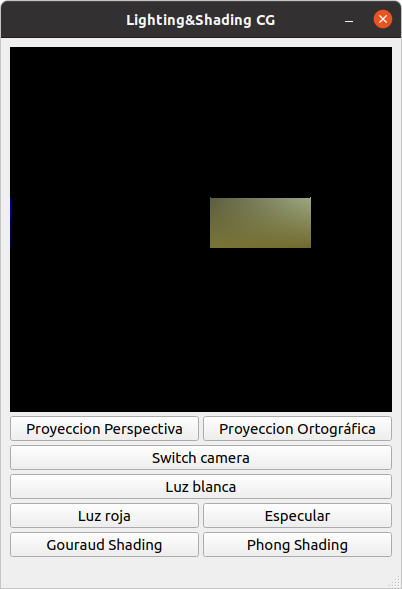
\includegraphics[scale=0.5]{images/gui.png}
\caption{Interfaz gráfica del programa}
\end{figure}

Al presionar \textit{switch camera} se cambia la posición de la cámara de cam1 a cam2.

Los botones \textit{Luz blanca}, \textit{Luz Roja} y \textit{Especular} encienden o apagan las luces correspondientes. EL programa inicia con todas las luces activas.



\section{Programa en ejecución}

\begin{figure}[H]
\centering
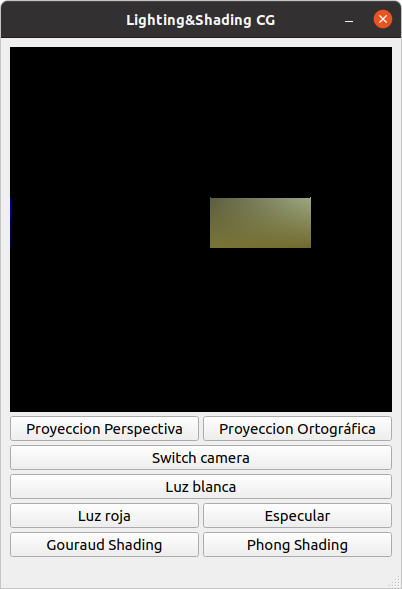
\includegraphics[scale=0.5]{images/ej1.png}
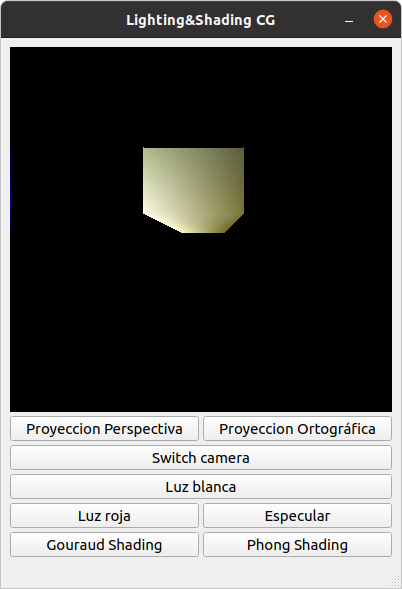
\includegraphics[scale=0.5]{images/ej2.png}
\caption{Cuboide con bordes y con rellenado. Proyectado en perspectiva}
\end{figure}


\begin{figure}[H]
\centering
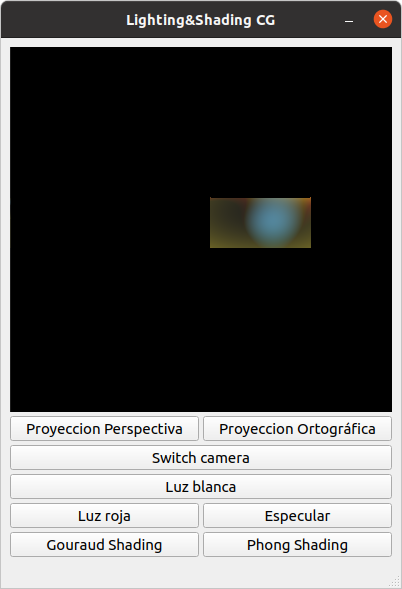
\includegraphics[scale=0.5]{images/ej3.png}
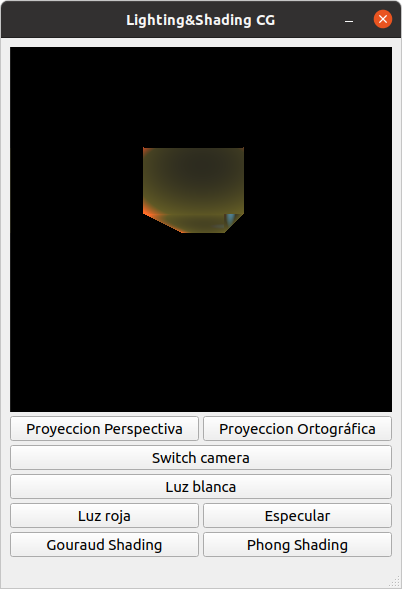
\includegraphics[scale=0.5]{images/ej4.png}
\caption{Cuboide con bordes y con rellenado. Proyectado en perspectiva}
\end{figure}



\begin{figure}[H]
\centering
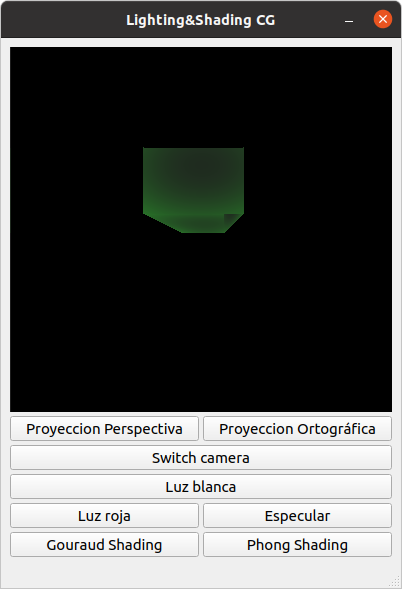
\includegraphics[scale=0.5]{images/ej6.png}
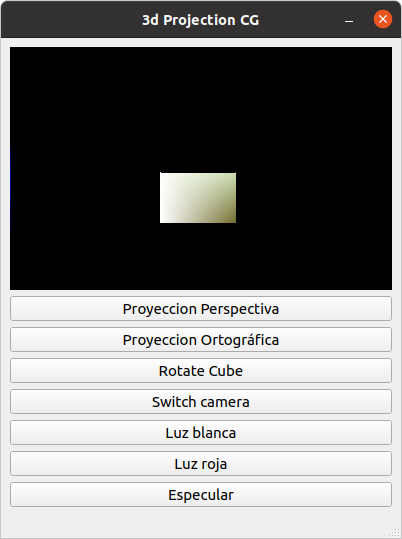
\includegraphics[scale=0.5]{images/ej7.png}
\caption{Cuboide con bordes y con rellenado. Proyección Ortográfica}
\end{figure}


\begin{thebibliography}{99}


\bibitem{dda} Marchese. Image creation and Graphic primitives ($https://csis.pace.edu/~marchese/CG_Rev/L4/cg_l4.htm$)

\bibitem{fill} Funkhouser. 2D rendering Pipeline ($https://www.cs.princeton.edu/courses/$$\\$$archive/fall99/cs426/lectures/pipeline$)

\bibitem{bb} Upssala Universit. Introduction to polygons. ($http://www.it.uu.se/edu/course/homepage$\\$/grafik1/ht06/Lectures/L02/LinePolygon/x_polyd.htm$)

\end{thebibliography}


\end{document}